\chapter{Visual Perception}

\section*{Making extremes stand out}

\begin{figure}[h]
    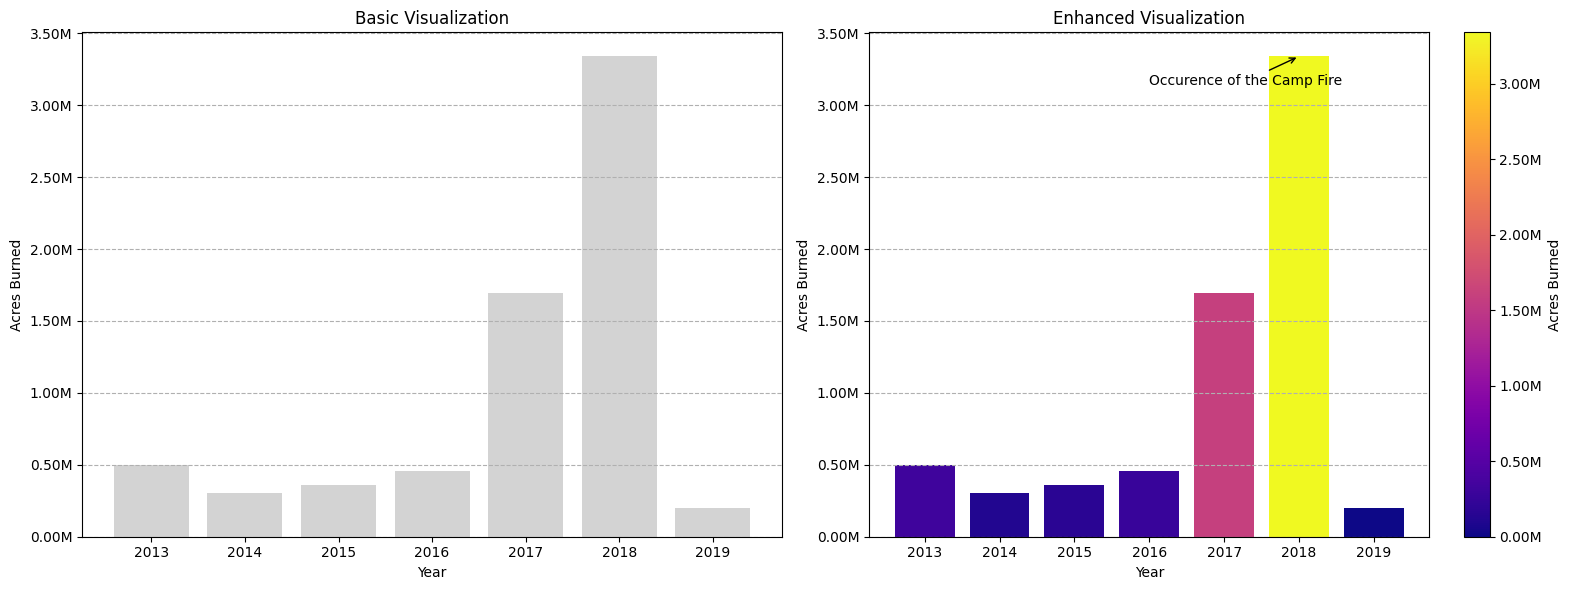
\includegraphics[width=\linewidth]{Images/figures/color_enhanced.png}
    \caption{Color enhancement comparison}
    \label{fig:colorenhanced}
\end{figure}

On the left, we have the \textbf{Basic Visualization} without colors and annotations, using a uniform light gray color for all bars.

On the right, we have the \textbf{Enhanced Visualization} with color gradients representing the intensity of acres burned, the year with the maximum acres burned highlighted in red, and an annotation providing context about the maximum value.

Of course one could say the first "Basic Visualization" is more than enough but the latter version even allows to capture the year of the most damage in a more dramatic way without having to examine axes and context closer.

\section*{3D and its perceptual problems}

\begin{figure}[h]
    \centering
    \begin{minipage}{.5\textwidth}
        \centering
        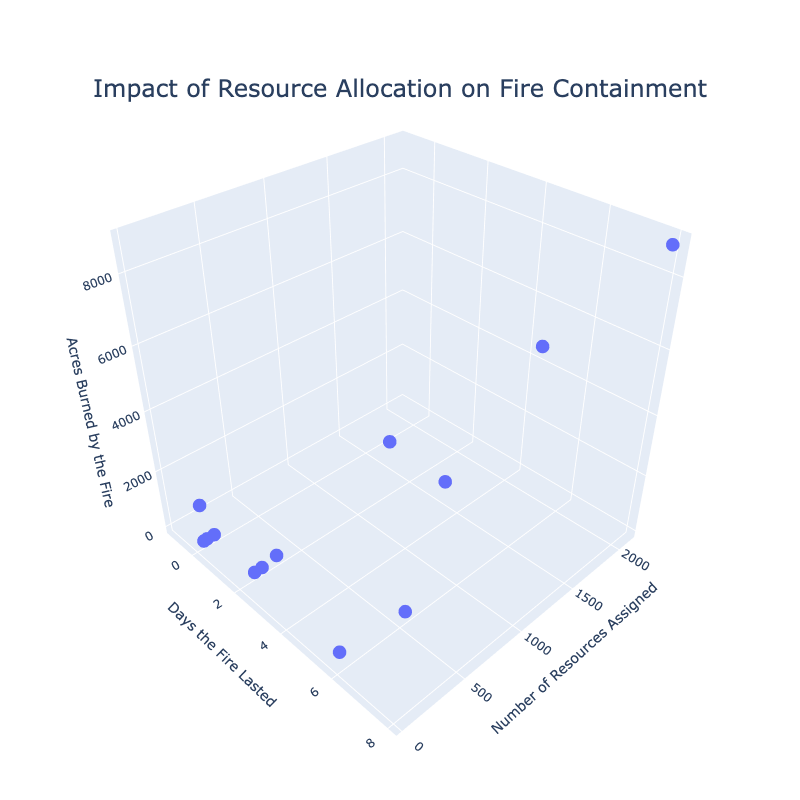
\includegraphics[height=6cm]{Images/figures/3d.png}
        \caption{3D Plot}
        \label{fig:plot1}
    \end{minipage}%
    \begin{minipage}{.5\textwidth}
        \centering
        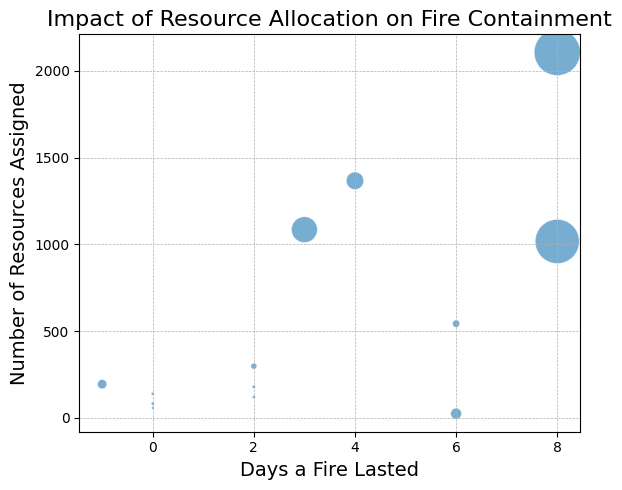
\includegraphics[height=6cm]{Images/figures/scatter_sizes.png}
        \caption{Simplified Plot}
        \label{fig:plot2}
    \end{minipage}
\end{figure}

2D plots are often preferred for clarity and simplicity. They can be easier to read, especially when printed or viewed on a flat medium like paper or a non-interactive display. 3D plots, on the other hand, can provide additional perspective and are excellent for displaying complex datasets with three distinct variables. However, without interactivity, 3D plots can become confusing and may not effectively communicate the data due to issues with perspective, such as occlusion (where parts of the graph obscure other parts) or distortion (where the angle of view can make certain dimensions appear different than they are). Here, the 2D plot shows the exact same data as the 3D plot but we made use of another property, the \textbf{scatter size}.

\section*{Counteracting Overlapping Data}

\begin{figure}[h]
    \centering
    \begin{minipage}{.5\textwidth}
        \centering
        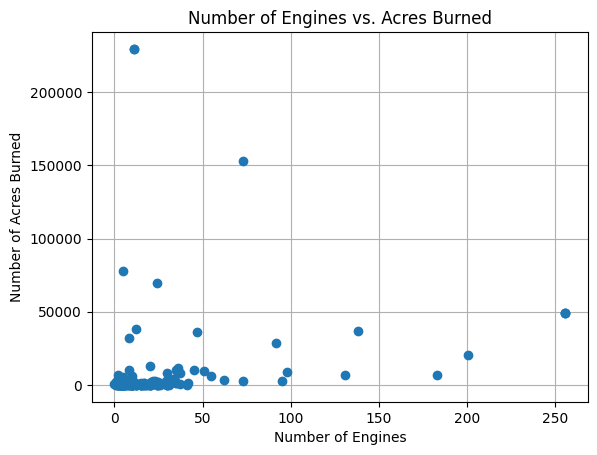
\includegraphics[height=6cm]{Images/figures/scatter_default.png}
        \caption{Default Scatter Plot}
        \label{fig:plot3}
    \end{minipage}%
    \begin{minipage}{.5\textwidth}
        \centering
        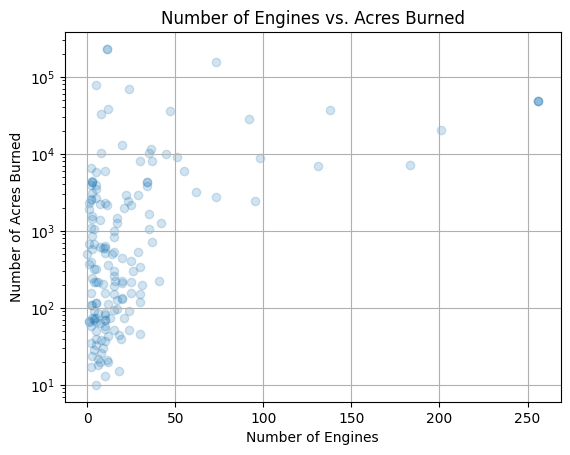
\includegraphics[height=6cm]{Images/figures/scatter_alpha_log.png}
        \caption{Enhanced Scatter Plot}
        \label{fig:plot4}
    \end{minipage}
\end{figure}

The data points are clustered at the lower end of the engines axis, indicating that most observations have a relatively low number of engines involved. Overlapping data points, particularly where the concentration of points is high, can obscure individual data values and may indicate a need for more sophisticated plotting techniques. Let's see how we can modify the \textbf{scatter plot} to see what actually lies behind the dense cluster of points.

Applying a lower alpha value to the scatter points, as shown in the right plot, helps to mitigate the issue of overlapping data points by making the points semi-transparent, which allows for the visualization of density in regions with high data point concentration. Furthermore, transforming the y-axis to a logarithmic scale spreads out the points along the vertical axis, providing a clearer view of the data across a wider range of values. However, this approach can make it more difficult to interpret the actual values, especially for those unfamiliar with logarithmic scales, as the scale compresses the data range and changes the perception of the distances between points. The reduced emphasis on individual, more transparent points can make it challenging to notice outliers or standalone points which could be significant. This trade-off in clarity for density versus emphasis on individual data points requires careful consideration when visualizing data to ensure accurate interpretation.